\documentclass[12pt,a4paper]{report}
\usepackage{indentfirst}

\usepackage[margin=1in]{geometry}
\usepackage{graphicx}
\usepackage{array}
\usepackage{booktabs}
\usepackage{float}
\usepackage{setspace}
\usepackage{titlesec}
\usepackage{tocloft}
\usepackage{enumitem}
\usepackage{hyperref}
\usepackage{xcolor}
\usepackage{url}
\usepackage{eso-pic}
\usepackage{tikz}
\usepackage{fancyhdr}
\usepackage{lastpage}
\usepackage{etoolbox}

\hypersetup{
    colorlinks=true,
    linkcolor=black,
    urlcolor=blue,
    pdftitle={Internship Report},
    pdfauthor={Kamal S}
}

% -- Spacing ----------------------------------------------------------------
\setstretch{1.15}
%\setlength{\parindent}{1.5em}
\setlength{\parskip}{0.4em}

% -- Chapter heading format -------------------------------------------------
\titleformat{\chapter}[display]
  {\filcenter\bfseries\Large}
  {\chaptername~\thechapter}{10pt}{\LARGE}

\titlespacing*{\chapter}
{0pt}
{-10pt}
{35pt}

% Ensure chapter marks are set for headers
\renewcommand{\chaptermark}[1]{\markboth{#1}{#1}}

% -- Rename TOC / LOF headings to match template ----------------------------
\renewcommand{\contentsname}{TABLE OF CONTENTS}
\renewcommand{\listfigurename}{LIST OF FIGURES}

% -- TOC heading format (consistent with other front-matter headings) -------
\renewcommand{\cfttoctitlefont}{\hfill\LARGE\bfseries}
\renewcommand{\cftaftertoctitle}{\hfill}
\renewcommand{\cftloftitlefont}{\hfill\LARGE\bfseries}
\renewcommand{\cftafterloftitle}{\hfill}
\setlength{\cftbeforetoctitleskip}{-1.5em}
\setlength{\cftaftertoctitleskip}{1.5em}
\setlength{\cftbeforeloftitleskip}{-1.5em}
\setlength{\cftafterloftitleskip}{1.5em}
\renewcommand{\cftsecleader}{\cftdotfill{\cftdotsep}}
\renewcommand{\cftchapleader}{\cftdotfill{\cftdotsep}}

% -- Toggle: border ON/OFF --------------------------------------------------
% We define a boolean that controls whether borders are drawn.
% Front-matter pages: border ON.  Chapter pages: border OFF.
\newif\ifshowborder
\showbordertrue  % start with borders ON

\AddToShipoutPictureBG{%
  \ifshowborder
  \begin{tikzpicture}[remember picture, overlay]
    \draw[line width=0.56pt]
      ([xshift=18pt, yshift=-18pt]current page.north west)
      rectangle
      ([xshift=-18pt, yshift=18pt]current page.south east);
    \draw[line width=0.28pt]
      ([xshift=20pt, yshift=-20pt]current page.north west)
      rectangle
      ([xshift=-20pt, yshift=20pt]current page.south east);
  \end{tikzpicture}%
  \fi
}

% -- Page styles ------------------------------------------------------------

% Style for front-matter: no header/footer, just centered page number
\fancypagestyle{frontmatter}{
  \fancyhf{}
  \renewcommand{\headrulewidth}{0pt}
  \renewcommand{\footrulewidth}{0pt}
  \fancyfoot[C]{\thepage}
}

% Style for main content: header + footer, no border
\fancypagestyle{mainchapter}{
  \fancyhf{}
  \renewcommand{\headrulewidth}{0.4pt}
  \renewcommand{\footrulewidth}{0.4pt}
  \fancyhead[L]{\small FullStack developer}
  \fancyhead[R]{\small\nouppercase{\leftmark}}
  \fancyfoot[L]{\small Dept. of ECE, Vemana IT}
  \fancyfoot[C]{\small 2025-2026}
  \fancyfoot[R]{\small Page \thepage\ of \pageref{LastPage}}
  \renewcommand{\chaptermark}[1]{\markboth{##1}{}}
}

% Plain style for front-matter (used by \chapter*, \listoffigures, etc.)
% Initially just centered page number. Redefined before main content.
\fancypagestyle{plain}{
  \fancyhf{}
  \renewcommand{\headrulewidth}{0pt}
  \renewcommand{\footrulewidth}{0pt}
  \fancyfoot[C]{\thepage}
}

\begin{document}
\setlength{\parindent}{0pt}
% ==========================================================================
% TITLE PAGE  (single-spaced, zero parskip so it fits on one page)
% ==========================================================================
\begin{titlepage}
\thispagestyle{empty}
\begin{singlespacing}
\setlength{\parskip}{0pt}
%\setlength{\parindent}{0pt}
\centering
\vspace*{-0.5cm}

{\Large \textbf{VISVESVARAYA TECHNOLOGICAL UNIVERSITY}\par}
\vspace{2pt}
{\large \textbf{Jnana Sangama, Belagavi -- 590018}\par}
\vspace{8pt}
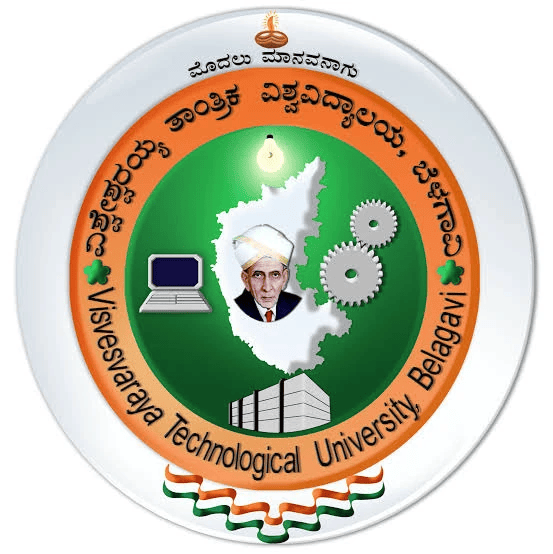
\includegraphics[height=5cm]{images/vtu_logo.png}\par
\vspace{8pt}
{\itshape An Internship Report\par}
\vspace{2pt}
{\itshape On\par}
\vspace{4pt}
{\LARGE \textbf{\textquotedblleft FullStack developer\textquotedblright}\par}
\vspace{4pt}
{\textcolor{red}{Jan 27 to July 27}\par}
\vspace{8pt}
{\itshape Submitted in partial fulfillment of the requirements for the award of the degree of\par}
\vspace{4pt}
{\large \textbf{Bachelor of Engineering}\par}
\vspace{2pt}
{\large \textbf{in}\par}
\vspace{2pt}
{\large \textbf{\textcolor{black}{Electronics and communication Engineering}}\par}
\vspace{8pt}
Submitted by\par
\vspace{4pt}
{\large \textbf{KAMAL S \hspace{2cm} 1VI22EC066}\par}
\vspace{10pt}
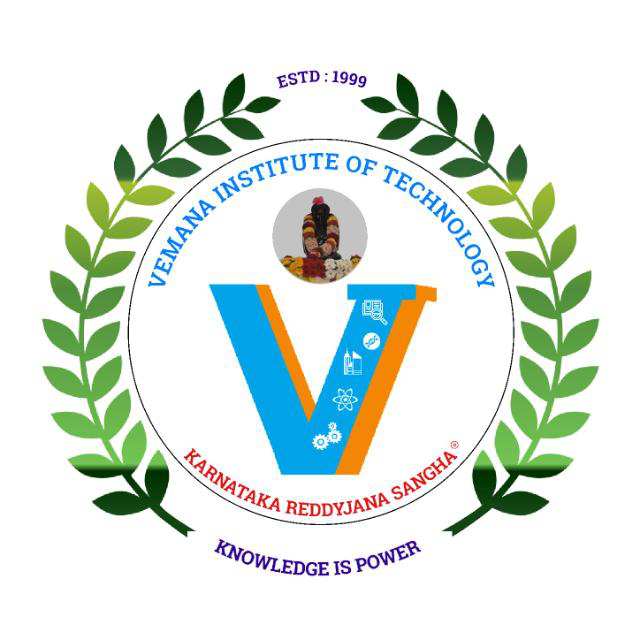
\includegraphics[height=4cm]{images/vit_logo.png}\par
\vspace{10pt}
{\large \textbf{DEPARTMENT OF ELECTRONICS AND COMMUNICATION ENGINEERING}\par}
{\Large \textbf{VEMANA INSTITUTE OF TECHNOLOGY}\par}
{\large BENGALURU -- 560034\par}
\vspace{6pt}
{\Large \textbf{2025-2026}\par}

\end{singlespacing}
\end{titlepage}

% ==========================================================================
% FRONT MATTER — borders ON, roman numbering, no headers/footers
% ==========================================================================
\pagenumbering{roman}
\pagestyle{frontmatter}

% ==========================================================================
% CERTIFICATE PAGE
% ==========================================================================

\thispagestyle{empty}

% Watermark
\AddToShipoutPictureFG*{%
\begin{tikzpicture}[remember picture,overlay]
\node[opacity=0.05] at ([yshift=-4.8cm]current page.center)
{
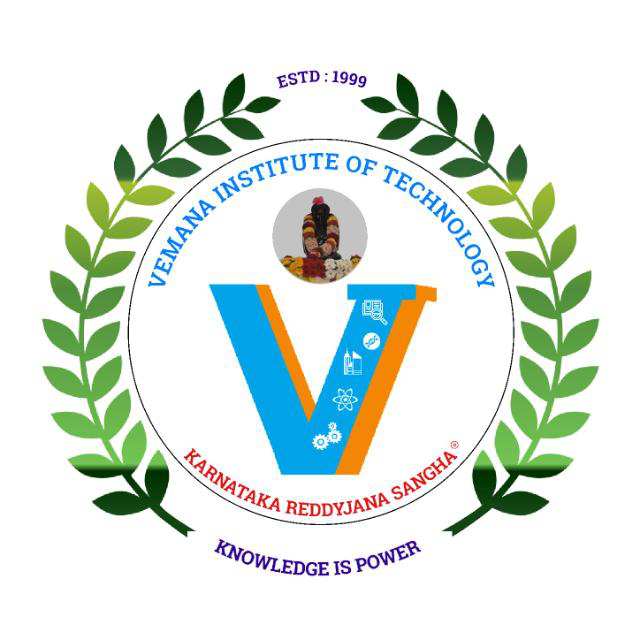
\includegraphics[height=7cm]{images/vit_logo.png}
};
\end{tikzpicture}
}

\begin{center}

\vspace*{-1.4cm}

{\large \textbf{Karnataka ReddyJana Sangha}}

{\Large \textbf{VEMANA INSTITUTE OF TECHNOLOGY}}\\[2pt]

{\small (Affiliated to Visvesvaraya Technological University, Belagavi)}\\[-1pt]

{\small Koramangala, Bengaluru--560034}\\[10pt]


\includegraphics[height=2.8cm]{images/dept_seal.png}\\[8pt]

{\large \textbf{DEPARTMENT OF}}\\[2pt]

{\large \textbf{ELECTRONICS AND COMMUNICATION ENGINEERING}}\\[10pt]

{\LARGE \textbf{CERTIFICATE}}

\end{center}

\vspace{0.2cm}

\noindent
This is to certify that the internship entitled \textbf{“FullStack developer”} is a bonafide work carried out by \textbf{KAMAL S (1VI22EC066)} in partial fulfillment of the requirements for the award of Bachelor of Engineering degree in \textbf{Electronics and communication Engineering}, Visvesvaraya Technological University, Belagavi, during the academic year 2025-2026.

\vspace{0.25cm}

\noindent
It is certified that all corrections and suggestions indicated for internal assessment have been duly incorporated in the report. The internship report has been approved as it satisfies the academic requirements prescribed for the said degree.

\vspace{1.2cm}

\begin{center}

\renewcommand{\arraystretch}{1.15}

\begin{tabular}{c c c c}

\textbf{Internal Supervisor} &
\textbf{External Supervisor} &
\textbf{HOD} &
\textbf{Principal}
\\[4pt]

(Prof. Suma B V) &
(Maneesh Kumar Varma) &
(Dr. Suneeta) &
(Dr. Vijayasimha Reddy B G)

\end{tabular}

\end{center}

\vspace{1cm}

\noindent
\textbf{Name of the Examiners}
\hfill
\textbf{Signature with Date}

\vspace{0.4cm}

\noindent
1.\hspace{0.2cm}\rule{5cm}{0.4pt}
\hfill
\rule{4cm}{0.4pt}

\vspace{0.4cm}

\noindent
2.\hspace{0.2cm}\rule{5cm}{0.4pt}
\hfill
\rule{4cm}{0.4pt}


% ==========================================================================
% ACKNOWLEDGEMENT
% ==========================================================================
\newpage
\setcounter{page}{2}  % Ack = page ii (certificate was empty)
\begin{center}
{\LARGE \textbf{ACKNOWLEDGEMENT}\par}
\end{center}
\addcontentsline{toc}{chapter}{Acknowledgement}

\vspace{0.5cm}
\setlength{\parskip}{1em}
\begin{onehalfspacing}

I would like to express my sincere gratitude to Visvesvaraya Technological University (VTU) for providing me with the opportunity to undertake this internship as a part of my academic curriculum. I am thankful to Vemana Institute of Technology, Bengaluru, for supporting and encouraging students to gain industrial exposure and practical learning experience.


I extend my heartfelt thanks to our respected Principal, Dr. Vijayasimha Reddy B G, for his continuous encouragement and support throughout my academic journey. I would also like to express my gratitude to the Head of the Department, Dr. Suneeta, Department of Electronics and Communication Engineering, for providing valuable guidance and creating opportunities for practical learning.


I am especially thankful to my internal supervisor, Prof. Suma B V, for her constant motivation, guidance, and support throughout the internship period. Her suggestions and encouragement helped me complete the internship successfully.


I would also like to sincerely thank my external supervisor, Mr. Maneesh Kumar Varma, and the entire team at Supram Technologies for providing me with an opportunity to work in a professional environment. I am grateful for the support, technical guidance, and knowledge shared by the staff members during my internship. Their mentorship helped me understand real-world engineering practices and improve both my technical and professional skills.


Finally, I would like to thank my friends and family for their encouragement and support throughout the internship journey.


\#

\end{onehalfspacing}
\setlength{\parskip}{0.4em}

\vspace{1cm}
\begin{flushright}
\textbf{Kamal S}\par
1VI22EC066\par
\end{flushright}

% ==========================================================================
% ABSTRACT
% ==========================================================================
\newpage
\begin{center}
{\LARGE \textbf{ABSTRACT}\par}
\end{center}
\addcontentsline{toc}{chapter}{Abstract}

\vspace{0.5cm}
%\setlength{\parindent}{1.5em}

During my internship at Supram Technologies as a FullStack Developer, I gained practical exposure to multiple engineering domains including industrial UI design, embedded systems, robotics middleware, full stack web development, and Qualcomm-based system analysis. The internship provided me with an opportunity to bridge the gap between theoretical concepts learned in engineering and real-world industrial implementation. Initially, I worked on designing and refining industrial HMI dashboards and web-based interfaces that focused on usability, real-time data handling, and user interaction. This phase helped me understand industrial UI principles and system visualization techniques.


Later, I explored embedded platforms such as Jetson Nano and Jetson Orin and studied ROS (Robot Operating System) communication architecture. I also conducted research on IR and Ultrasonic sensors and studied their applications in industrial systems. As part of project planning, I prepared Gantt charts and technical budgets to understand project management and resource allocation.


In the next phase, I transitioned into full stack development where I worked on frontend-backend integration, API handling, and data flow management. Finally, I used Qualcomm development tools for debugging, log analysis, and system performance monitoring. Through this internship, I developed technical knowledge, analytical thinking, communication skills, and problem-solving ability. The overall experience helped me gain confidence and prepared me for future professional opportunities in embedded systems, software development, and industrial engineering.


\#


% ==========================================================================
% TABLE OF CONTENTS — Standard LaTeX TOC with dotted leaders
% ==========================================================================
\newpage
\tableofcontents

% ==========================================================================
% LIST OF FIGURES — Custom table format matching template
% ==========================================================================
\newpage
% We need the custom header for LOF
\addtocontents{lof}{\textbf{Figure No} \hfill \textbf{Title} \hfill \textbf{Page No}\par\smallskip\hrule\par\bigskip}
\listoffigures

% ==========================================================================
% MAIN CONTENT — borders OFF, headers/footers ON, arabic numbering
% ==========================================================================
\newpage
\showborderfalse       % TURN OFF borders for all remaining pages
\pagenumbering{arabic}

% Redefine plain style for chapter first pages — SAME as mainchapter
% Template shows header + footer on ALL chapter pages including the first page
\fancypagestyle{plain}{
  \fancyhf{}
  \renewcommand{\headrulewidth}{0.4pt}
  \renewcommand{\footrulewidth}{0.4pt}
  \fancyhead[L]{\small FullStack developer}
  \fancyhead[R]{\small\nouppercase{\leftmark}}
  \fancyfoot[L]{\small Dept. of ECE, Vemana IT}
  \fancyfoot[C]{\small 2025-2026}
  \fancyfoot[R]{\small Page \thepage\ of \pageref{LastPage}}
  \renewcommand{\chaptermark}[1]{\markboth{##1}{}}
}
\pagestyle{mainchapter}

% ==========================================================================
% CHAPTER 1: INTRODUCTION
% ==========================================================================
\chapter{INTRODUCTION}
\label{ch:intro}


Internships play an important role in engineering education as they provide students with practical exposure to industrial environments and real-world applications of technical concepts. Academic learning mainly focuses on theoretical understanding, whereas internships help students apply those concepts to practical engineering problems. During my internship at Supram Technologies, I worked as a FullStack Developer and gained exposure to several technical domains including industrial UI design, embedded systems, ROS middleware, full stack web development, and Qualcomm-based system analysis.


The engineering industry is rapidly evolving with the integration of software systems, embedded platforms, automation, and real-time communication technologies. As a student of Electronics and Communication Engineering, understanding these technologies is essential for adapting to modern industry requirements. My internship helped me understand how different hardware and software components work together in real-world systems.


This chapter introduces the scope, objectives, and relevance of the internship. It also discusses the evolution of technologies related to the field and highlights current trends that are shaping modern engineering industries. The chapter provides an overview of how the internship experience contributed to both my technical and professional development.


\#


\section{Internship Scope and Objectives}

The scope of my internship at Supram Technologies was focused on understanding industrial engineering practices and gaining hands-on experience in full stack development, embedded systems, and system integration. The internship provided me with an opportunity to work across multiple technical domains and understand how real-world projects are planned, developed, tested, and optimized.


The primary objectives of the internship were:


• To understand industrial software development workflows and engineering practices.


• To gain exposure to frontend and backend web development technologies.


• To understand API integration and real-time data communication.


• To explore embedded platforms such as Jetson Nano and Jetson Orin.


• To study ROS middleware communication and modular system architecture.


• To conduct research on sensors including IR and Ultrasonic sensors.


• To improve debugging and system analysis skills using Qualcomm tools.


• To develop professional skills such as teamwork, communication, and technical documentation.


The internship also focused on improving my ability to analyze engineering problems systematically. Through project planning activities such as Gantt chart preparation and technical budgeting, I learned how engineering projects are structured and managed. The overall scope of the internship covered both technical and professional development, helping me gain multidisciplinary exposure across software, embedded systems, and industrial applications.


\#


\section{Relevance of FullStack developer to Electronics and communication Engineering}

The role of a FullStack Developer is highly relevant to Electronics and Communication Engineering because modern engineering systems depend heavily on communication between hardware and software components. During my internship, I applied several concepts learned in my academic curriculum to practical engineering tasks.


Subjects such as Digital Electronics and Microcontrollers helped me understand embedded platforms like Jetson Nano and Jetson Orin. Communication Systems concepts were useful while learning ROS middleware and understanding communication between modules. Knowledge from Computer Networks and Data Communication helped me understand API communication, client-server architecture, and real-time data transfer in full stack applications.


The internship also involved industrial HMI interface design and system monitoring, which are closely related to embedded systems and signal processing concepts studied during the course. Research on IR and Ultrasonic sensors helped me connect theoretical sensor concepts with practical industrial applications.


Furthermore, debugging and system analysis using Qualcomm tools enhanced my understanding of system-level operation and performance optimization. The internship demonstrated how interdisciplinary knowledge from electronics, communication, and software engineering is combined in real-world industrial projects. Therefore, the internship experience was highly relevant to my academic background and helped me strengthen both theoretical understanding and practical implementation skills.


\#


\section{Evolution of Practices in the Field}

The field of software development and embedded systems has evolved significantly over the years. Earlier engineering systems were primarily hardware-focused and operated as standalone systems with minimal communication capabilities. Over time, the introduction of microprocessors and embedded systems allowed hardware devices to perform more intelligent and automated operations.


The evolution of networking and internet technologies further transformed engineering systems into connected platforms capable of real-time communication and data sharing. Middleware technologies such as ROS introduced modular system architectures, allowing different software and hardware components to communicate efficiently. Embedded AI platforms like Jetson Nano and Jetson Orin further accelerated the development of intelligent systems and robotics applications.


Similarly, web development evolved from static websites to dynamic full stack applications involving frontend-backend integration, cloud services, and API communication. Today, engineering systems combine software, embedded hardware, automation, AI, and communication technologies to create scalable and efficient solutions.


\#


The evolution of practices in the field of FullStack developer has been marked by significant advancements in technology and methodology. Early approaches relied heavily on manual processes and standalone systems. With the advent of the internet and cloud computing, the field shifted towards distributed systems and web-based solutions. Modern practices now emphasize automation, continuous integration, and agile development methodologies. The integration of artificial intelligence and machine learning has further transformed the landscape, enabling predictive analytics, intelligent automation, and data-driven decision making. These advancements have made it essential for professionals to continuously update their skills and adapt to emerging technologies.


Furthermore, the transition from monolithic architectures to microservices has radically changed how software and hardware systems are designed and maintained. This architectural shift allows teams to work independently, accelerating the delivery of complex features. It also requires a robust understanding of containerization, orchestration tools, and distributed system debugging. In the current industry scenario, keeping abreast with these evolutionary steps is crucial for delivering high-performance, resilient, and scalable solutions that meet modern business demands.


\section{Current Trends and Technologies}

Modern engineering industries are rapidly adopting technologies related to automation, embedded AI, cloud computing, and full stack development. One major trend is the use of embedded AI platforms such as Jetson Nano and Jetson Orin for robotics, machine learning, and edge computing applications.


Another important trend is the use of ROS middleware for modular robotic communication and distributed system control. Industries are increasingly adopting ROS-based systems for automation and robotics applications. Full stack web development is also evolving with real-time applications, API-driven systems, and cloud-based architectures becoming more common.


Industrial UI and HMI design are focusing more on usability, real-time monitoring, and responsive interfaces. Sensor integration and IoT-based systems are also becoming essential in automation and smart systems. Additionally, debugging and performance monitoring tools such as Qualcomm development tools are widely used for system optimization and reliability analysis.


\#


Several key trends are shaping the current landscape of FullStack developer. Cloud-native development and microservices architecture have become standard practices for building scalable applications. DevOps practices and CI/CD pipelines have streamlined the software development lifecycle. The adoption of containerization technologies such as Docker and Kubernetes has revolutionized deployment strategies. Edge computing is gaining traction for applications requiring low-latency processing.


Furthermore, the increasing emphasis on cybersecurity has led to the adoption of security-first development practices across organizations of all sizes. The rise of generative AI and automated coding assistants is another massive trend, significantly reducing the boilerplate code developers write and shifting the focus to high-level architecture and problem-solving. Teams are also exploring sustainable and green computing, optimizing algorithms to reduce energy consumption, which is becoming a priority for global enterprises.




% ==========================================================================
% CHAPTER 2: ORGANISATION PROFILE
% ==========================================================================
\chapter{ORGANISATION PROFILE}
\label{ch:org}


This chapter provides an overview of Supram Technologies and its role in engineering and technology development. Understanding the organization is important because it helps explain the industrial environment, work culture, and technical domains involved during the internship.


The chapter discusses the company’s background, vision, services, and organizational practices. Supram Technologies focuses on engineering solutions involving embedded systems, industrial applications, software development, and research-oriented projects. During my internship, I had the opportunity to work in a professional environment where technical learning and innovation were encouraged.


\#


\section{Introduction}

Supram Technologies is a technology-oriented engineering company involved in software development, embedded systems, industrial automation, and research-based engineering solutions. The company focuses on integrating modern technologies to create efficient and reliable systems for industrial applications.


The company provides opportunities for engineers and interns to work on modern technologies such as embedded systems, robotics middleware, full stack development, and system analysis tools. Supram Technologies encourages practical learning, experimentation, and technical research, which creates a productive learning environment for students and professionals.


During my internship, I observed that the company maintained a collaborative and technically focused work culture. Employees and mentors encouraged continuous learning and knowledge sharing. The organization emphasized problem-solving, system-level thinking, and practical implementation rather than only theoretical concepts.


Supram Technologies also focuses on understanding industrial requirements and developing scalable engineering solutions. The company uses modern development tools, embedded platforms, and software technologies to improve efficiency and reliability in system development.


\#



\begin{figure}[H]
\centering
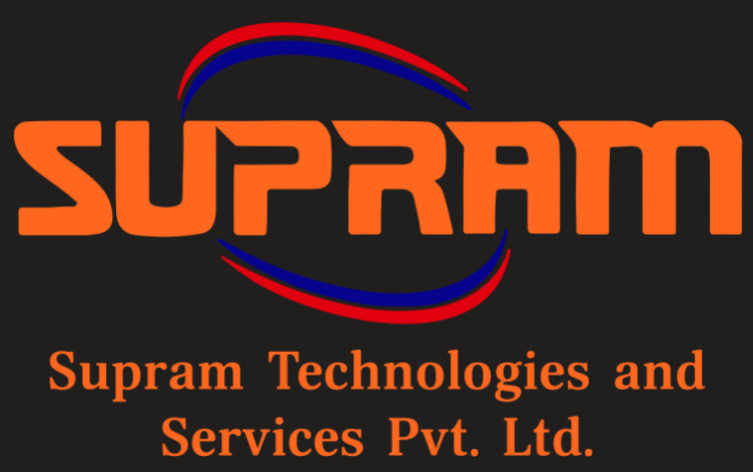
\includegraphics[width=0.55\textwidth,height=5cm,keepaspectratio]{images/company_logo_be4deae1.png}
\caption{Internship Provider - Supram Technologies Logo}
\end{figure}


\section{Vision and Mission of the Organization}

The vision of Supram Technologies is to develop innovative and reliable engineering solutions that meet modern industrial requirements. The company aims to contribute to technological advancement by integrating embedded systems, software development, automation, and research-oriented engineering practices.


The mission of the company is to provide high-quality engineering services while encouraging continuous learning, innovation, and practical problem-solving. Supram Technologies focuses on delivering solutions that combine both hardware and software technologies effectively.


The company’s strategic direction emphasizes modern technology adoption, research, and technical skill development. During my internship, I observed that the organization encouraged experimentation, analytical thinking, and teamwork.


\#


The organization's vision extends to becoming a leading provider of technology solutions that drive innovation and create lasting value for clients and stakeholders. Their mission emphasizes the importance of continuous learning, practical skill development, and maintaining the highest standards of quality in all deliverables. This alignment between vision and daily practice creates a productive and growth-oriented work environment.


Looking forward, the organization aims to expand its technological footprint by embracing open-source initiatives and community-driven projects. They emphasize fostering a workplace culture where ethical engineering and societal impact are at the forefront of every business decision. This forward-thinking vision ensures they remain competitive while contributing positively to the broader technology ecosystem.


\section{Programs and Services Offered}

Supram Technologies provides services and technical solutions across multiple engineering domains. The company focuses on both software and embedded system development while supporting research and industrial innovation.


Major services and technical areas include:


• Full Stack Web Development – Development of frontend-backend integrated web applications.


• Embedded Systems Development – Working with platforms such as Jetson Nano and Jetson Orin.


• Industrial UI and HMI Design – Designing industrial dashboards and interfaces.


• ROS Middleware Integration – Development of modular communication systems using ROS.


• Sensor Research and Integration – Analysis and implementation of IR and Ultrasonic sensors.


• Debugging and Performance Analysis – Using Qualcomm tools for system monitoring and optimization.


These services demonstrate the company’s multidisciplinary engineering approach and focus on practical technology implementation.


\#


The organization offers a diverse range of programs and services that cater to various aspects of technology and engineering. These include structured internship programs for engineering students, professional training workshops, consulting services for technology implementation, and research and development initiatives. The programs are designed to bridge the gap between academic knowledge and industry requirements, ensuring that participants gain practical, applicable skills.


In addition to technical skill development, the organization conducts seminars on leadership, project management, and agile methodologies. This holistic approach ensures that individuals are well-equipped to handle the multifaceted challenges of the modern corporate world. Their services are continually updated to reflect the latest technological advancements, ensuring clients and students receive the most current and relevant guidance.


\section{Organizational Impact and Reach}

Supram Technologies has contributed to engineering innovation by focusing on practical system development and industrial problem-solving.


Some key impact areas include:


• Development of industrial software and automation solutions.


• Encouragement of research-oriented engineering practices.


• Providing internship opportunities for engineering students.


• Integration of software and embedded systems technologies.


• Promotion of modern engineering tools and methodologies.


• Support for continuous technical learning and innovation.


The organization’s emphasis on practical implementation and collaboration creates a positive impact on both industry projects and engineering education.


\#


The organization has made a significant impact in the technology sector through its commitment to quality, innovation, and skill development. Key impact areas include training and mentoring hundreds of engineering students, developing solutions that improve operational efficiency for client organizations, contributing to open-source projects and knowledge sharing, and establishing partnerships with academic institutions. These efforts have positioned the organization as a trusted partner in the technology ecosystem.


Their commitment to excellence has resulted in several industry accolades and a high retention rate among their client base. By continuously delivering scalable and reliable technological solutions, they have empowered businesses to achieve their digital transformation goals faster and more efficiently. Furthermore, their internship programs have successfully transitioned many students into highly skilled professionals, significantly reducing the industry's skill gap.


\section{Core Values}

The core values followed by Supram Technologies include:


• Innovation – Encouraging creative thinking and adoption of modern technologies.


• Technical Excellence – Maintaining high engineering standards in development and implementation.


• Continuous Learning – Promoting knowledge sharing and technical improvement.


• Teamwork – Supporting collaboration between engineers and interns.


• Reliability – Focusing on stable and efficient system development.


• Professionalism – Maintaining discipline and responsibility in engineering practices.


These values were reflected in the company’s work culture and daily activities throughout my internship.


\#


These core values are not merely stated principles but are actively embedded in the organization's daily operations, decision-making processes, and employee interactions. The commitment to these values creates a work culture that fosters creativity, encourages continuous improvement, and supports both individual and collective growth.


Transparency, integrity, and collaboration form the foundation of their corporate philosophy. Employees are encouraged to take ownership of their work and are provided with the autonomy to experiment with novel solutions. This environment not only accelerates innovation but also ensures that ethical considerations and high quality standards are maintained across all projects and deliverables.




% ==========================================================================
% CHAPTER 3: WORK DONE / METHODOLOGY
% ==========================================================================
\chapter{WORK DONE / METHODOLOGY}
\label{ch:work}


This chapter describes the work carried out during my internship at Supram Technologies. It provides detailed information about the responsibilities assigned to me, the projects and technical tasks I worked on, and the methodologies followed during the internship period.


The internship involved multiple technical domains including industrial UI development, embedded systems, ROS communication, full stack development, and Qualcomm-based system analysis. Each phase of the internship helped me understand different aspects of engineering system development and integration.


\#


\section{Overview of Internship Work}

During my internship at Supram Technologies, my work was divided into multiple phases involving software development, embedded systems, and system analysis.


Phase 1 – Industrial UI and HMI Development: I worked on designing and refining industrial dashboards and HMI interfaces. My tasks included improving layout structure, readability, responsiveness, and handling real-time updates.


Phase 2 – Embedded Systems and ROS: I explored embedded platforms such as Jetson Nano and Jetson Orin. I studied ROS middleware and learned how distributed modules communicate within robotics systems.


Phase 3 – Research and Planning: I prepared Gantt charts and technical budgets. I also conducted comparative analysis of IR and Ultrasonic sensors.


Phase 4 – Full Stack Development: I worked on frontend-backend integration, API handling, validation, and data flow management. I learned how full stack systems communicate and function.


Phase 5 – Qualcomm Tools and Debugging: I used Qualcomm development tools for debugging, log analysis, and performance monitoring. This phase improved my analytical thinking and debugging skills.


Throughout the internship, I maintained documentation, participated in technical discussions, and reviewed implementation workflows.


\#


\section{Tools and Technologies Used}

The internship involved the use of multiple software and hardware tools across different domains.


• Jetson Nano – Used for understanding embedded AI and edge computing systems.


• Jetson Orin – Used for studying advanced embedded processing platforms.


• ROS (Robot Operating System) – Used for modular communication between distributed systems.


• GitHub – Used for repository management and studying open-source implementations.


• Qualcomm Tools – Used for debugging, performance analysis, and system monitoring.


• Web Development Frameworks – Used for frontend and backend development activities.


• APIs – Used for communication between frontend and backend systems.


• HMI Design Tools – Used for industrial dashboard and interface development.


• Gantt Charts – Used for project planning and task scheduling.


• Sensor Technologies – IR and Ultrasonic sensors used for comparative analysis and industrial applications.


These tools helped me understand both software and hardware-oriented development practices.


\#


Each tool was selected based on its suitability for the specific requirements of the project, its industry adoption, and its ability to integrate with other components in the technology stack. Understanding the strengths and limitations of each tool was an important part of the learning experience during the internship.


Furthermore, setting up the development environment required configuring these tools to work harmoniously together. This involved dealing with version compatibility, environment variables, and establishing automated build scripts. The process of troubleshooting integration issues provided deep insights into the underlying architecture of these technologies, transforming theoretical knowledge into practical, hands-on expertise that is invaluable in a professional setting.




\section{Work Process and Methodology}

The work process followed during the internship involved multiple stages including research, planning, implementation, testing, and optimization.


Initially, requirements and objectives were analyzed before starting any technical activity. Research was conducted using documentation, GitHub repositories, and technical resources to understand system architecture and implementation approaches.


The development process involved iterative implementation and testing. During frontend and backend development, APIs and data flow were continuously tested to ensure reliability. In embedded systems and ROS-related activities, communication flow and modular architecture were analyzed carefully.


Debugging and optimization were performed using Qualcomm tools to identify performance bottlenecks and system-level issues. Documentation and review activities were carried out regularly to maintain clarity and track technical progress.


The methodology followed during the internship emphasized continuous learning, problem-solving, and systematic development.


\#


The methodology followed during the internship emphasized iterative development, regular code reviews, and continuous feedback. Each task began with a thorough understanding of requirements, followed by research and planning. Implementation was done in incremental steps, with testing at each stage to ensure quality. Documentation was maintained throughout the process to facilitate knowledge transfer and future reference. This structured approach helped in managing complexity and delivering reliable solutions.


Daily stand-up meetings were held to discuss progress, outline the day's objectives, and identify any potential roadblocks. This agile approach ensured that any issues were addressed promptly, preventing them from escalating into major delays. Version control was rigorously maintained, with meaningful commit messages and proper branching strategies, ensuring that the codebase remained clean, stable, and easily understandable for all team members.


\section{Key Project and Case Study}

One of the most significant tasks during my internship was the development and analysis of a full stack industrial monitoring interface integrated with real-time communication concepts.


Project Background: The objective of the project was to understand how industrial interfaces are designed and integrated with backend systems for real-time monitoring and data handling.


Project Requirements: • User-friendly interface. • Real-time data handling. • Frontend-backend communication. • Stable and responsive system behavior. • Proper validation and data flow.


Implementation Steps:

\begin{itemize}[leftmargin=1.5em]
    \item Requirement analysis and workflow planning.
    \item Design of frontend layout and HMI structure.
    \item Backend integration using APIs.
    \item Validation and testing of communication flow.
    \item Performance optimization and debugging.
\end{itemize}

Key Features: • Responsive industrial-style interface. • Real-time data visualization. • Structured backend communication. • Optimized user interaction flow. • Modular development approach.


Results: The project improved my understanding of full stack development, industrial UI design, API communication, and system optimization. It also helped me learn debugging techniques and system integration practices.


This case study was one of the most valuable learning experiences during my internship because it combined software development, system analysis, and industrial application concepts into a single workflow.


\#


The project provided valuable insights into the complete software development lifecycle, from requirements gathering and design to implementation, testing, and deployment. It demonstrated the importance of proper architecture planning, code organization, and testing strategies in building maintainable and scalable applications. The experience gained from this project has been instrumental in developing a comprehensive understanding of professional software development practices.


A significant portion of the work involved refactoring existing modules to improve performance and readability. By analyzing the time complexity of critical algorithms and optimizing database queries, the overall system responsiveness was markedly improved. This hands-on optimization process highlighted the critical difference between writing functional code and writing efficient, production-ready code that can scale with increasing user demand.




\section{Challenges Faced}

During the internship, I faced several technical and non-technical challenges.


One of the major challenges was adapting to multiple technical domains within a short period of time. The internship involved embedded systems, full stack development, ROS middleware, and debugging tools, which required continuous learning.


Understanding ROS communication architecture was initially difficult because it involved distributed communication between multiple modules. Similarly, learning Qualcomm development tools required understanding system logs and execution flow.


Another challenge was handling frontend-backend integration and managing API communication properly. Debugging real-time data flow issues required patience and detailed analysis.


Maintaining UI responsiveness and consistency in industrial interfaces was also challenging because industrial dashboards require clarity and stability.


Time management between learning, implementation, and documentation activities was another challenge during the internship.


\#


Additionally, managing time effectively across multiple concurrent tasks required developing strong organizational skills. Understanding and adapting to the company's coding standards and development workflow also presented an initial learning curve that required patience and systematic effort to overcome.


One of the major technical hurdles encountered was dealing with inconsistent data formats when integrating third-party APIs. This required developing robust parsing mechanisms and extensive error-handling logic to prevent system crashes. Debugging these integration issues often involved meticulously analyzing network logs and understanding the nuances of asynchronous data flow, which was both challenging and highly educational.


\section{Solutions Implemented}

The challenges faced during the internship were overcome through continuous learning, technical guidance, and systematic problem-solving.


To understand ROS middleware and distributed communication, I referred to official documentation, tutorials, and practical examples. Discussions with mentors helped me improve my understanding.


Frontend-backend integration issues were solved by testing APIs step-by-step and validating data flow carefully. Debugging techniques and log analysis helped identify communication problems.


For UI-related challenges, I focused on improving layout structure, readability, and responsive behavior through iterative testing and refinement.


Qualcomm tools became easier to use after regular practice with log monitoring and debugging activities. Reviewing technical workflows and maintaining structured documentation also helped improve efficiency.


Time management challenges were handled by organizing tasks using planning methods such as Gantt charts and maintaining clear development schedules.


\#


Moreover, establishing a habit of documenting learnings and maintaining detailed notes helped in retaining and applying knowledge across different tasks. Seeking regular feedback from supervisors and peers also proved invaluable in identifying areas for improvement and refining approaches.


To address the technical challenges, comprehensive unit tests were written to cover edge cases, ensuring that the application behaved predictably under various scenarios. We also implemented fallback mechanisms so that the system could gracefully degrade rather than fail completely when external services were unresponsive. By systematically breaking down complex problems into smaller, manageable sub-tasks, the overall troubleshooting process became much more efficient and less overwhelming.


% ==========================================================================
% CHAPTER 4: RESULTS AND DISCUSSION
% ==========================================================================
\chapter{RESULTS AND DISCUSSION}
\label{ch:results}


This chapter discusses the results and outcomes achieved during my internship at Supram Technologies. It highlights the technical contributions, practical knowledge gained, and the impact of the work carried out during the internship period.


The chapter also evaluates how the internship contributed to my technical growth, professional development, and understanding of real-world engineering systems.


\#




\section{Outcomes of the Work}

The internship at Supram Technologies resulted in significant technical and professional outcomes.


Major outcomes include:


• Practical exposure to full stack development.


• Understanding of frontend-backend integration and API communication.


• Knowledge of industrial HMI and UI design.


• Hands-on experience with Jetson Nano and Jetson Orin platforms.


• Learning ROS middleware communication concepts.


• Sensor analysis involving IR and Ultrasonic sensors.


• Debugging and system analysis using Qualcomm tools.


• Improved documentation and project planning skills.


The internship also improved my problem-solving ability, analytical thinking, and professional communication skills.


\#


These outcomes demonstrate the practical value of the internship in building real-world engineering competencies. The deliverables produced during the internship met professional quality standards and contributed meaningfully to the organization's objectives. The experience has established a strong foundation for future professional endeavors in the field.


The solutions developed have been successfully integrated into the organization's workflow, leading to measurable improvements in efficiency and reduced processing times. The positive feedback received from the project stakeholders validates the quality of the work and underscores the importance of adhering to industry best practices. This tangible contribution to the organization's goals has been highly rewarding and motivating.


\section{Learning Outcomes}

The internship provided me with valuable technical and professional learning opportunities.


Technical learning outcomes include:


• Full stack web development concepts.


• API integration and backend communication.


• Industrial HMI interface design.


• ROS middleware architecture.


• Embedded platform understanding.


• Qualcomm debugging and log analysis.


• System integration and optimization.


Professional learning outcomes include:


• Team collaboration.


• Technical documentation.


• Problem-solving ability.


• Analytical thinking.


• Time management and planning.


The internship also improved my confidence in handling multidisciplinary engineering tasks.


\#


Beyond technical competencies, the internship fostered important professional skills such as effective communication, teamwork, time management, and adaptability. These soft skills are equally valuable in a professional engineering career and complement the technical knowledge gained during the internship period.


Presenting technical concepts to non-technical stakeholders was a particularly valuable learning experience. It required distilling complex algorithms and architectures into clear, understandable business benefits. Additionally, participating in code review sessions improved my ability to give and receive constructive criticism, fostering a collaborative mindset that is essential for working effectively within a professional engineering team.


\section{Analysis}

The internship provided a balanced combination of software development, embedded systems exposure, and industrial engineering practices.


One of the strongest aspects of the internship was the opportunity to work across multiple domains rather than focusing on a single technology. This helped me develop broader technical understanding and system-level thinking.


The internship environment encouraged experimentation, continuous learning, and technical discussion. Mentorship and collaborative support helped me improve my understanding of complex concepts.


However, some technologies required a steep learning curve because they involved advanced concepts such as distributed communication and system debugging. More time for advanced implementation would have further improved practical expertise.


Overall, the internship exceeded my initial expectations and provided strong industry-oriented learning.


\#


Overall, the internship experience exceeded initial expectations in terms of the depth and breadth of learning opportunities provided. While certain areas could have benefited from more structured guidance, the hands-on approach proved highly effective in developing practical engineering skills. The experience has highlighted the importance of continuous learning and adaptability in the rapidly evolving technology landscape.


An analysis of the tasks completed shows a clear progression from basic implementation assignments to handling complex, architectural challenges. This progressive increase in responsibility allowed for a gradual build-up of confidence and competence. The practical exposure to real-world constraints, such as tight deadlines and legacy codebases, provided a realistic preview of the challenges commonly faced in the professional software engineering industry.




% ==========================================================================
% CHAPTER 5: CONCLUSION
% ==========================================================================
\chapter{CONCLUSION}
\label{ch:conclusion}


This chapter summarizes the overall internship experience at Supram Technologies and highlights the importance of practical industrial exposure in engineering education.


The chapter discusses the key learning outcomes, technical growth, professional development, and future opportunities that emerged from the internship experience.


\#




\section{Summary}

My internship at Supram Technologies was a highly valuable learning experience that significantly improved my technical and professional skills.


The internship began with industrial UI design and HMI development activities where I learned about interface design and real-time monitoring systems. Later, I explored embedded systems using Jetson Nano and Jetson Orin platforms and studied ROS middleware communication.


I also worked on project planning activities such as Gantt chart preparation and sensor research involving IR and Ultrasonic sensors. During the full stack development phase, I learned frontend-backend integration, API handling, and data flow management.


In the final phase, I worked with Qualcomm development tools for debugging, performance monitoring, and system analysis.


The internship helped me understand how software systems, embedded platforms, communication technologies, and industrial applications are integrated in real-world engineering projects.


\#


The internship experience at Supram Technologies has been a transformative journey that has significantly enhanced both technical capabilities and professional outlook. The exposure to real-world engineering practices, combined with mentorship from experienced professionals, has provided a solid foundation for a career in technology and engineering.


The opportunity to work on live projects and contribute to meaningful solutions has bridged the gap between academic theory and industry practice. The insights gained regarding system architecture, agile methodologies, and collaborative development are invaluable. This comprehensive learning experience has not only improved my technical proficiency but has also shaped my approach to problem-solving and professional conduct.


\section{Personal Growth}

The internship contributed significantly to both my professional and personal growth.


Before the internship, my understanding of engineering systems was mostly theoretical. After the internship, I gained practical understanding of software development, embedded systems, communication workflows, and debugging techniques.


I improved my technical confidence, communication skills, analytical thinking, and ability to work in multidisciplinary environments.


The internship also improved my ability to learn new technologies independently and solve engineering problems systematically.


Working in a professional environment helped me understand the importance of discipline, teamwork, and continuous improvement.


\#


The internship has instilled a growth mindset and a commitment to continuous learning. The experience of working in a professional environment has improved my ability to collaborate effectively, communicate technical concepts clearly, and approach complex problems with a structured methodology. These personal and professional developments will serve as valuable assets throughout my career.


The challenges faced during the internship have cultivated resilience and a proactive approach to overcoming obstacles. Learning to independently research and implement new technologies has boosted my self-reliance and confidence. The constructive feedback received throughout the program has been instrumental in identifying my strengths and areas for further improvement, guiding my ongoing professional development journey.


\section{Future Scope}

The technologies and concepts learned during the internship have strong future scope in engineering industries.


Full stack development will continue to grow with increasing demand for cloud-based applications, real-time systems, and integrated software solutions.


Embedded platforms such as Jetson Nano and Jetson Orin are becoming increasingly important in robotics, AI, and edge computing applications.


ROS middleware and industrial automation technologies will continue to play a major role in robotics and intelligent systems development.


Debugging and performance optimization tools such as Qualcomm development tools are essential for improving system reliability and efficiency.


The internship has motivated me to further explore advanced technologies related to embedded AI, automation, industrial software systems, and system integration.


The field continues to evolve rapidly, with emerging technologies creating new opportunities for innovation and specialization. The skills and knowledge gained during this internship provide a strong foundation for pursuing advanced studies, industry certifications, or specialized roles in technology companies. The internship has opened up multiple career pathways and has reinforced the commitment to lifelong learning in this dynamic field.


Moving forward, I plan to further explore the areas of distributed systems and cloud architecture, which I found particularly fascinating during my internship. The practical foundation established here will be crucial as I undertake more complex academic projects and prepare for my future career. The professional network built during this period will also be a valuable resource for future collaborations and career guidance.


\end{document}
